\documentclass[11pt]{article}
\usepackage{geometry} 
\geometry{margin=1in}
\geometry{a4paper} 


\usepackage{textcomp}
\usepackage{booktabs}
\usepackage{array}
\usepackage{paralist}
\usepackage{verbatim} 
\usepackage{subfigure}
\usepackage{graphicx,caption}
\usepackage{placeins}
\usepackage{lipsum}
\usepackage{xcolor}
\usepackage{dcolumn}
\usepackage{sectsty}
\allsectionsfont{\sffamily\mdseries\upshape}
\usepackage{gensymb,amsmath,mathtools,amssymb}
\usepackage{flafter}
%\usepackage{parskip}
\usepackage[utf8]{inputenc}
\usepackage[english]{babel}
\usepackage{tocbibind}
\usepackage[toc,page]{appendix}
\captionsetup{width=\linewidth}
\usepackage{bm}
\usepackage{url}
\usepackage{hyperref}
\usepackage{ar}


\hypersetup{
    colorlinks=true,
    linkcolor=blue,
    filecolor=magenta,      
    urlcolor=cyan,
    pdftitle={Design of the Glass Frog},
    bookmarks=true,
    pdfpagemode=FullScreen,
}

\newcommand{\eqn}[1]{\begin{equation}#1\end{equation}}
\newcommand{\eqnalign}[1]{\begin{align*}#1\end{align*}}

\newcommand{\half}{\frac{1}{2}}


\graphicspath{{./figs/}}


\title{Design and Loads Analysis for  the Glass Frog}
\author{Devansh Agrawal}
%\date{} 


\begin{document}

\maketitle


\section{Introduction}

The Glass Frog is a small high-powered rocket designed to showcase the capabilities of generative design. It is a technology demonstrator to demonstrate the ability to use cheap and easily available manufacturing processes to build and fly a rocket. 

In particular, the idea is to develop a small L1 scale rocket that has an organic, generatively designed airframe. It is to be 3D printed, with some laser cut parts where appropriate. It should be able to handle all the major load cases of a typical flight, carrying a small electronics payload and camera, launched in a conventional manner using a launch rail, and be recovered using a standard single deployment mechanism. 

In this document, my concept of this rocket is presented, and the input loads on the rocket are also calculated. This documentation and all the relevant scripts can be found in the Github repository for this work: \url{https://github.com/icl-rocketry/glass_frog_design}

\section{Concept}

A rough sketch of the rocket is in \autoref{fig:concept}. 

%\FloatBarrier
\begin{figure}[tbhp]
   \centering
   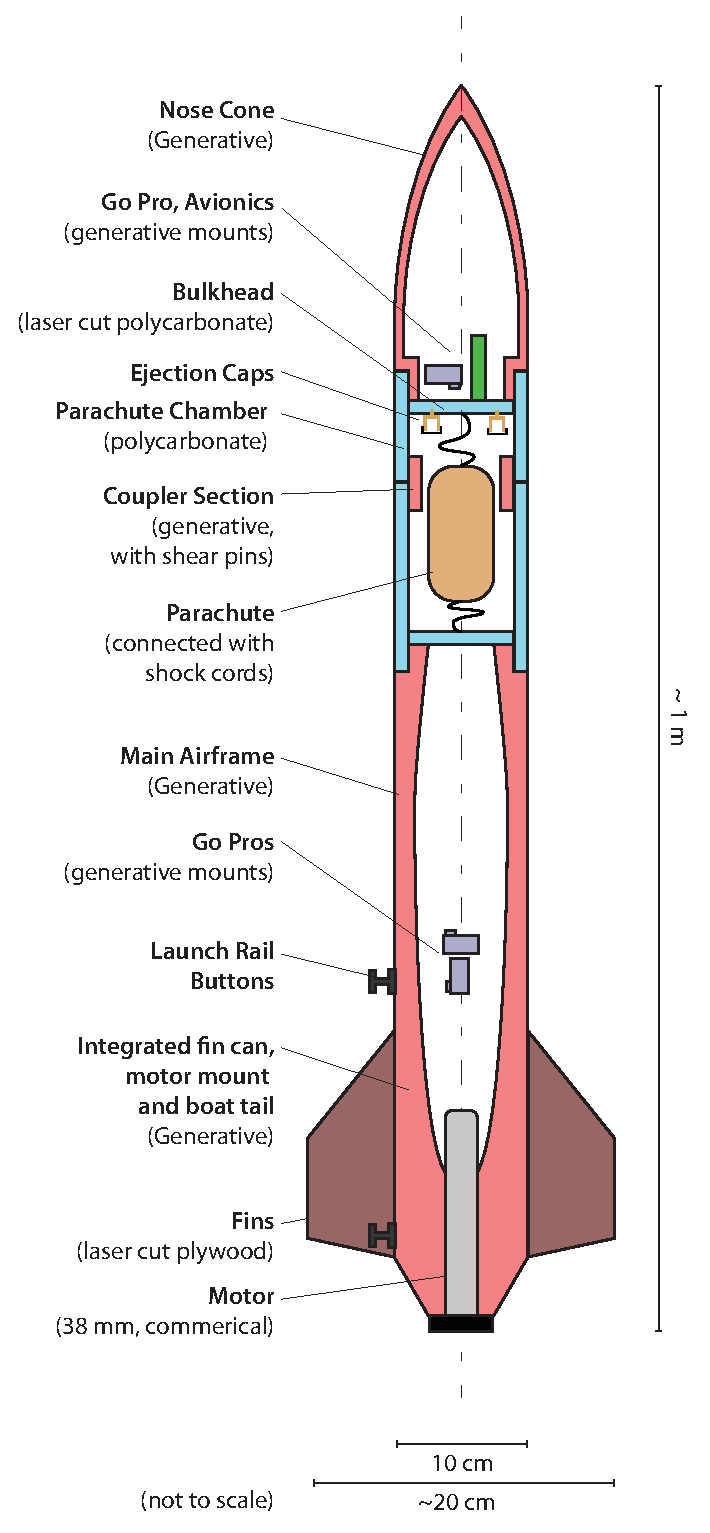
\includegraphics[width=0.7\textwidth, height=0.8\textheight,keepaspectratio]{figs/conceptSketch.eps}
   \caption{Concept sketch for }
   \label{fig:concept}
\end{figure}
%FloatBarrier

To make the rocket cool and really highlight the design, the organic truss structure is to be visible from the outside of the rocket. As this will cause aerodynamic issues, I propose we use a thin transparent (non-structural plastic sheet) wrapped around the outside of the rocket. This way, the internals of the rocket should be visible, and if the structure is printed from a solid colour (black or red probably) it should really stand out. 

For the recovery system, a section of body tube needs to be able to hold pressure, shearing the nylon shear pins and separating the main body tube of the rocket. The presusre can be generated through 3 main methods:\footnote{Side deployment methods were not considered as they are fairly uncommon and present significant risk of zippering the rocket or not deploying successfully.}
\begin{itemize}
\item The ejection charge at the end of the motor
\item A black powder charge ignited using some control electronics.\footnote{Any standard altimeter with charge ignition methods should work. For instance the \href{http://www.perfectflite.com/SLCF.html}{StartoLogger}.}
\item A CO\textsubscript{2} canister that is punctured using some control electronics.\footnote{Using the \href{https://fruitychutes.com/buyachute/co2-ejection-system-c-20/peregrine-raptor-co2-system-kit-23-to-45-gram-p-183.html}{Peregrine Raptor CO2 System} for instance}
\end{itemize}

Since the primary airframe construction is unlikely to  hold the pressure due to any of these methods, we need to design a pressurisable compartment for the parachute, as seen in the concept figure. 

The fins need to be mounted securely to the body tube. To do so, some slots suitable to take the fins were designed. These two slots allow the fins to slide in, and secured using a few screws. This was done to ease the construction (fins + fin can are hard to print in most normally sized printers) and to allow the fins to the replaced with larger or smaller fins as needed later in the design process. 

The motor mount is to be integrated with the fin can, to reduce part count and potentially save mass. 


While the payload isn't critical to this rocket\footnote{usually the only reason you need the rocket is the payload}, I decided that the most suitable payload for this rocket is a bunch of logging equipment. Two GoPros are to be mounted in the nose, one looking to the side, and one looking down the rocket to be able to see the parachute deployment. In addition to this, we might mount a GoPro in the lower part of the rocket, to be able to see the fins clearly, and help identify any fluttering issues. The payload will also include the StratoLogger or Eggtimer to be able to cause the parachute deployment events.


\section{Loads}

The primary loads that need to be designed for the rocket are discussed here, essentially as inputs to Fusion360. 

\subsection{Compressive Loads}

The motor will be generating compressive loads in the rocket. As the rocket launches, it will see a compressive load in the body structure that is smaller than the motor thrust, however for this design process, it makes sense to size the main airframe compressive loads as though we were doing a static fire with the nose clamped in a wall.

The main selection of motors to consider are the small L1 certification motors. I chose 38mm diameter motors as they are relatively easy to get. A quick search of suitable motors shows the range of these motors, using the notebook \texttt{scripts/motorSelection.ipynb}. \autoref{tbl:all_HI_motors} shows all H and I class motors. However, its too large a range. I will filter it further, limiting to 38 mm motors produced by Cessaroni (which is basically the only supplier of motors we can get in the UK)) and the table is far more limited \autoref{tbl:suitable_motors}. Plotting the distributions is also helpful (\autoref{fig:suitable_motors}). There are only about 35 motors to choose from, and many of those are also unlikely to be useable. 


\begin{table}[tbhp]
   \centering
   \caption{Summary of all H or I class Motors}
\begin{tabular}{@{}rrrrrrr@{}}
\toprule
& Avg Thrust (N) & Max Thrust (N) & Impulse (Ns) & Burn Time (s) & Dia (mm)   & L (mm)     \\ \midrule
count        & 246 & 204     & 246  & 246 & 246 & 246 \\
mean         & 242.08   & 390.19     & 370.27  & 2.05   & 37.01  & 331.15 \\
std          & 162.90   & 456.24     & 139.96  & 1.43   & 6.92   & 180.20 \\
min          & 42.20    & 63.70      & 160.80  & 0.31   & 24.00  & 69.00  \\
25\%         & 135.32   & 191.97     & 247.00  & 1.20   & 29.00  & 203.00 \\
50\%         & 211.00   & 293.00     & 352.00  & 1.71   & 38.00  & 290.00 \\
75\%         & 296.54   & 454.51     & 490.83  & 2.31   & 38.00  & 368.00 \\
max          & 1335.00  & 5808.00    & 640.00  & 9.00   & 54.00  & 992.00 \\ \bottomrule
\end{tabular}
   \label{tbl:all_HI_motors}
\end{table}


\begin{table}[tbhp]
   \centering
   \caption{Summary of all suitable Motors (Cessaroni, 38mm)}
\begin{tabular}{@{}rrrrrrr@{}}
\toprule
& Avg Thrust (N) & Max Thrust (N) & Impulse (Ns) & Burn Time (s) & Dia (mm)   & L (mm)     \\ \midrule
count        & 35    & 33      & 35   & 35 & 35   & 35  \\
mean         & 264.65   & 308.81     & 411.61  & 1.99  & 38.0  & 259.65\\
std          & 161.89   & 172.61     & 126.70  & 1.20  & 0.0    & 61.46  \\
min          & 55.20    & 94.50      & 232.40  & 0.520  & 38.0   & 185.00 \\
25\%         & 152.70   & 197.90     & 286.00  & 1.70  & 38.0   & 186.00 \\
50\%         & 223.39   & 260.60     & 394.60  & 1.88  & 38.0   & 245.00 \\
75\%         & 324.12   & 379.50     & 527.46  & 2.15  & 38.0   & 302.50 \\
max          & 805.30   & 932.50     & 636.10  & 7.51  & 38.0   & 367.00\\ \bottomrule
\end{tabular}
   \label{tbl:suitable_motors}
\end{table}

%\FloatBarrier
\begin{figure}[tbhp]
   \centering
   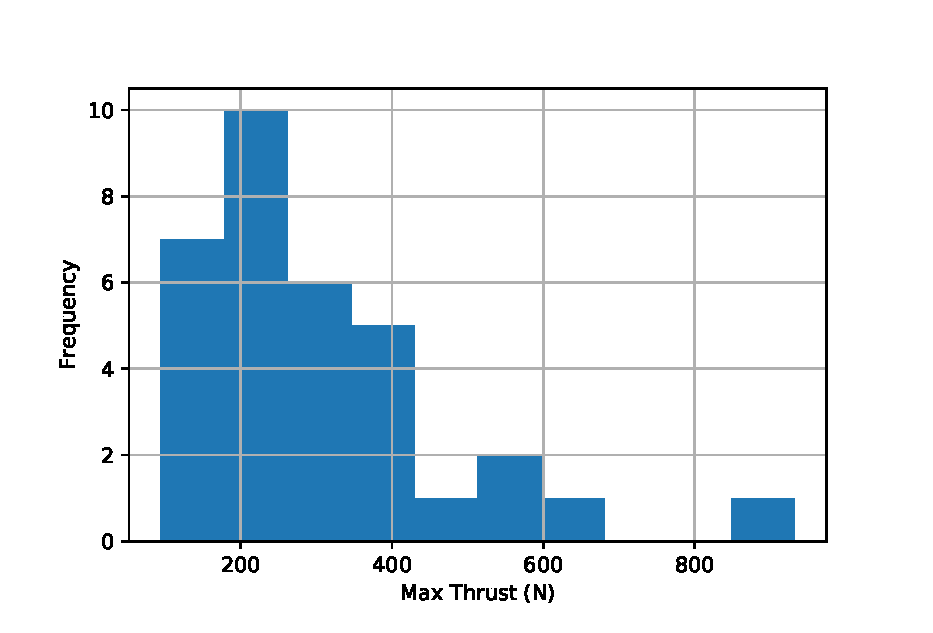
\includegraphics[width=0.45\linewidth]{figs/Max_Thrust_Distribution.eps}
    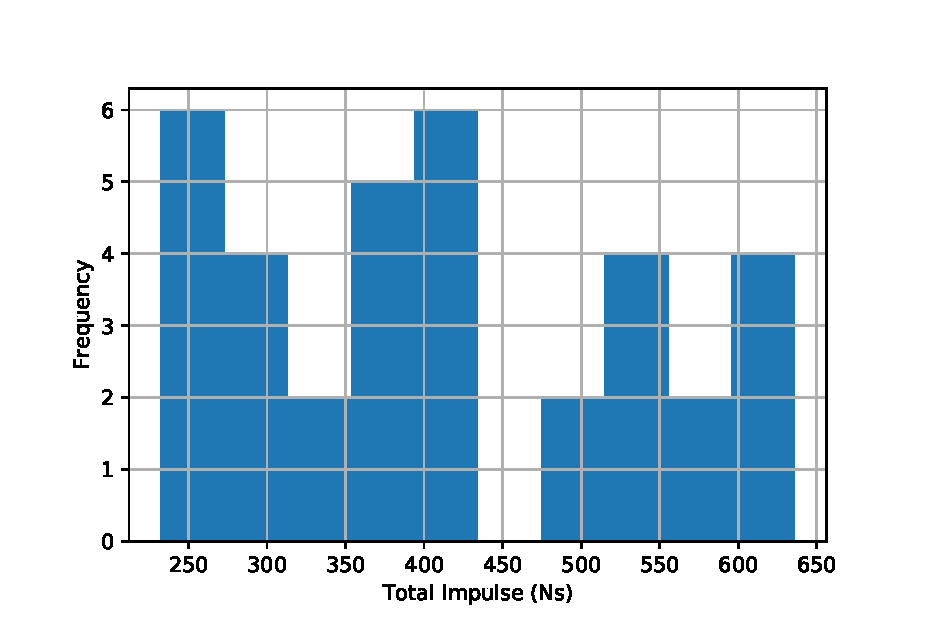
\includegraphics[width=0.45\linewidth]{figs/total_impulse_Distribution.eps}
    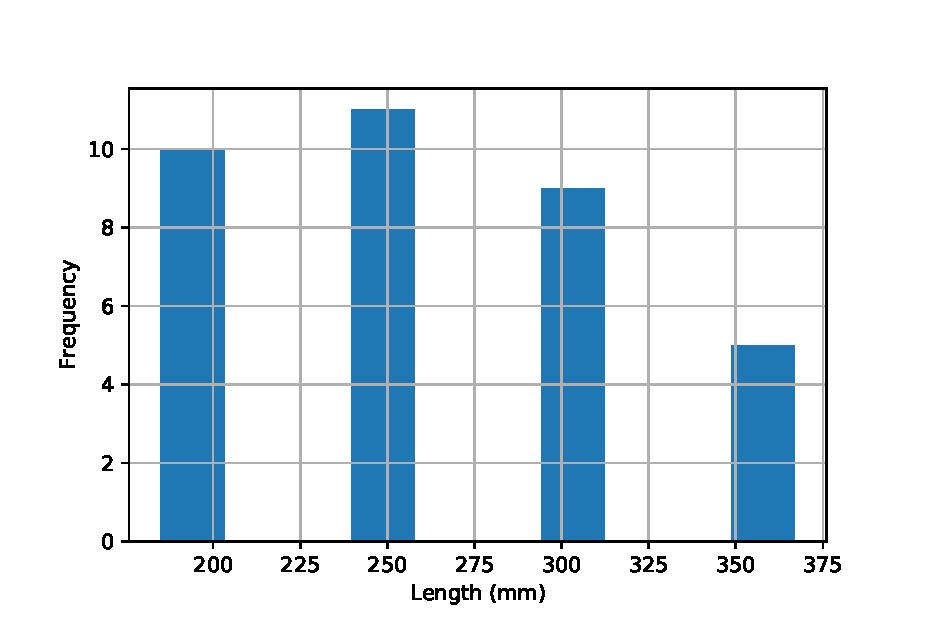
\includegraphics[width=0.45\linewidth]{figs/Length_Distribution.eps}
    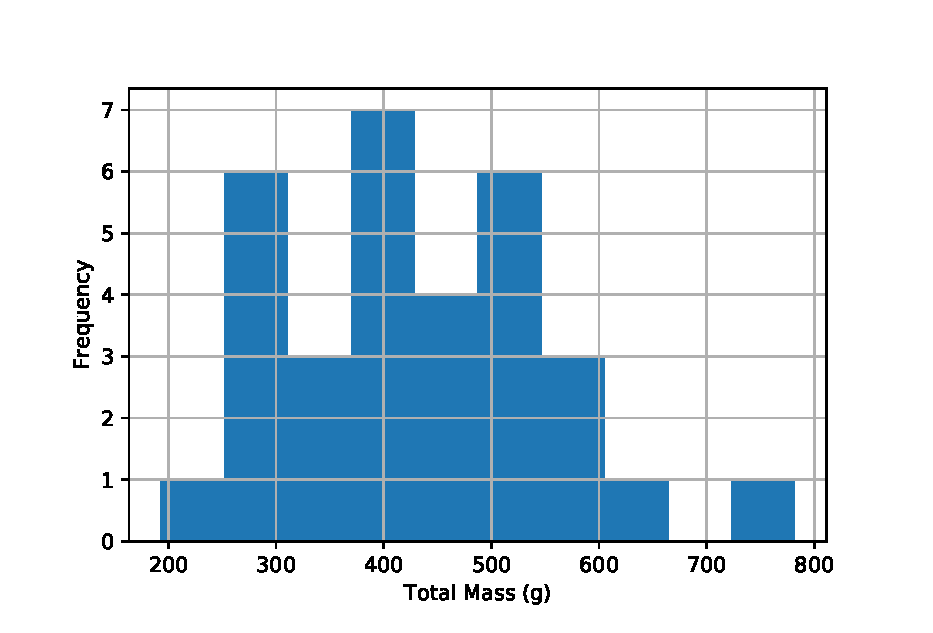
\includegraphics[width=0.45\linewidth]{figs/total_weight_Distribution.eps}
   \caption{Distribution of key motor parameters for in range of suitable motors.}
   \label{fig:suitable_motor_distribution}
\end{figure}
%FloatBarrier

Nonetheless, we can design for the most relevant cases, using the information that is in the table and figures. 

\begin{itemize}
\item Motor Diameter: 38 mm
\item Motor Length: upto 320 mm
\item Max Thrust:  650 N
\item Max Wet Mass of Motor: 700 g
\end{itemize}

To allow the structure to be resistant to off-axis loading, we allow this compressive thrust force to be applied within a 5\degree margin from the centre-line. 

\subsection{Fin loads}

A trapezoidal, flat plate fin is the easiest to analyse and manufacture. It's planform geometry is defined by the root chord, tip chord, and span. Further, it has a thickness and various material properties. For the purposes of determining the aero load, we can assume that the fin is rigid, and that it only imparts a root bending moment, shear forces and drag forces. 

The fin can be modelled as a thin beam, with loads at each section due to the chord being at some angle of attack. We can assume thin, flat plate theory, giving a lift coefficient of $2\pi \alpha$ where $\alpha$ is the angle of attack in radians. The analytic expressions are derived using Mathematica. 

The fin's generate a normal force, which is the lift force (\autoref{fig:fin_drawing}). Mandell \cite{mandell1973topics} showed that this force can be assumed to be acting at the fins centre of pressure, and has magnitude (for each fin)

\eqn{
C_{N\alpha1} = \frac{1}{\beta} K \frac{\AR \left(\frac{c_r + c_t}{r_t}\right)\left( \frac{b}{r_t}\right) }{2 + \sqrt{4 + \frac{\AR}{\cos \Gamma_c}} } \approx \frac{C_{N1}}{\alpha}
}

where 
\eqnalign{
C_{N1} & \quad \text{ is the lift force coefficient on a single fin}\\
C_{N\alpha1} &\equiv \frac{dC_{N1}}{d\alpha} \approx \frac{C_{N1}}{\alpha}  \quad \text{ is the lift force coefficient slope on a single fin}\\
\beta &=\sqrt{1-M_\infty^2} \quad \text{is the Prandtl-Glauert compressibility correction}\\
M_\infty & \quad \text{is the free stream mach number}\\
K &= 1 + \frac{1}{\tau} \quad \text{ is the fin-body interference correction}\\
\tau &= \frac{b + r_t}{r_t} \quad \text{ is the relative size of the fins}\\
\AR&=\frac{2 b}{c_r + c_t} \quad \text{ is the aspect ratio of the fin}\\
c_r &\quad  \text{is the root chord}\\
c_t & \quad \text{is the tip chord}\\
r_t & \quad \text{is the radius of the body tube}\\
b & \quad \text{is the span of the fin, measured from the fin root to the fin tip}\\
\Gamma_c & \quad \text{is the center-line sweep of the fins}
}

and this equation is valid for 3 or 4 fins. 
The location of the centre of pressure (see \autoref{fig:fin_drawing}) is
\eqn{
Z_{cp} = \frac{x_t}{3} \left(\frac{c_r + 2 c_t}{c_r + ct}\right) + \frac{1}{6} \left(c_r + c_t - \frac{c_r c_t}{c_r + c_t}\right)
}
\eqn{
Y_{cp} = r_t + \frac{b}{3} \left(\frac{c_r + 2 c_t}{c_r + c_t}\right)}
where $x_t$ is the longitudinal distance from the leading edge of the root to the tip. 

This set of equations has been implemented in the notebook \texttt{scripts/finForces.ipynb} using the fin class defined in \texttt{scripts/fin.py}.


%\FloatBarrier
\begin{figure}[tbhp]
   \centering
   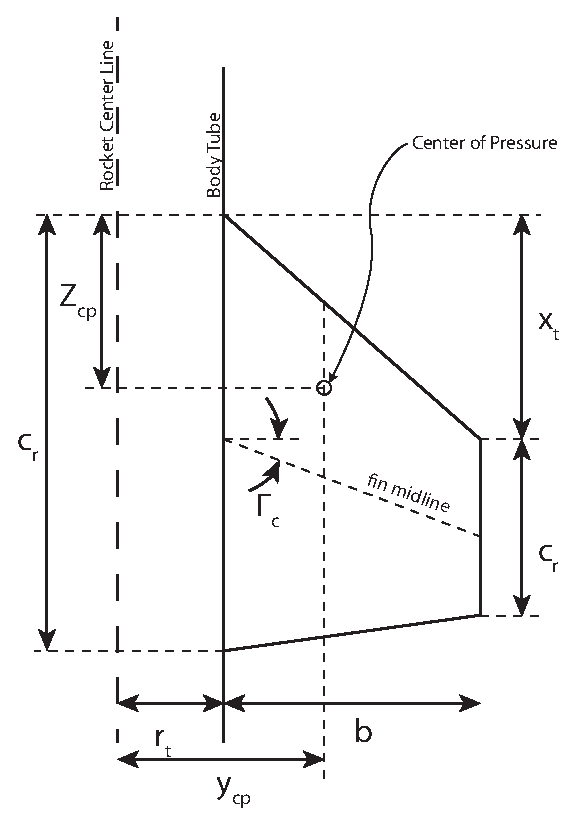
\includegraphics[width=0.5\linewidth]{figs/fin_drawing.eps}
   \caption{Fin dimensions and centre of pressure.}
   \label{fig:fin_drawing}
\end{figure}
%FloatBarrier


To use this to estimate the maximum lift force on a single fin, we need an estimate on the maximum dynamic pressure and the maximum angle of attack on the fins. Normally this requires a flight simulation using a tool like openRocket, but here I will claim experience to get a number. 

We can size the Glass Frog by assuming:
\begin{itemize}
\item Max Speed: Mach 0.4, V = 136 m/s 
\item Max Gust Speed: 9 m/s  \cite{aspire_space_loads}. 
\item $\rho=$1.225 kg/m\textsuperscript{3} (assumed constant with altitude for simplicity)
\end{itemize}

Therefore, the lift on the fin is 
\eqn{N = \half \rho V_\infty^2 C_{N\alpha1} \alpha A = \half \rho V_\infty V_\text{gust} C_{N\alpha1} A} 

where
\eqnalign{
N &\quad \text{is the lift force at the centre of pressure}\\
\rho &\quad \text{is the air density}\\
V_\infty & \quad \text{is the flight speed}\\
\alpha & \quad \text{is the angle of attack in radians}\\
V_\text{gust} & \quad \text{is the gust speed}\\
A & \quad \text{is the area of the fin}
}

and therefore the root bending moment is 
\eqn{M = N (y_{cp} - r_t)}


\subsection{Launch Forces}

We need to figure out the forces on the launch lugs as the vehicle is launched.

\subsection{Shock cord forces}

When the parachute deploys there will be some shock loads in the structure, and we need to figure out how these can be encoded. 


\newpage
\bibliographystyle{unsrt}
\bibliography{biblio}

\end{document}























